\documentclass[11pt,a4paper]{article}
\usepackage[T1]{fontenc}
\usepackage{lmodern}
\usepackage[margin=2.5cm]{geometry}
\usepackage{amsmath,amssymb}
\usepackage{graphicx}
\usepackage{booktabs}
\usepackage{caption}
\usepackage[numbers,sort&compress]{natbib}
\usepackage[hidelinks]{hyperref}
\usepackage{xurl}
\usepackage[section]{placeins}
\usepackage{xcolor}
\captionsetup{font=small,labelfont=bf}
\graphicspath{{figures/}}
\newcommand{\BTO}{BaTiO$_3$}
\newcommand{\dt}{d_{33}}
\newcommand{\Fp}{F_{\mathrm{polar}}}

\title{Interfacial Polar-Phase Nucleation and Piezoelectric Coupling in PVDF--Metal Oxide Nanocomposites for Energy Harvesting: A Physics-Based Modeling Framework}
\author{[Author names and affiliations]}
\date{}

\begin{document}
\maketitle

\begin{abstract}
We present a first-order, physics-based modeling framework for poly(vinylidene fluoride) (PVDF)/metal-oxide nanocomposite energy harvesters. The framework chains five steps: phase quantification, interphase geometry, dielectric mixing, piezoelectric coupling of 0--3 composites, and the electrical output of a lossy harvester under a resistive load. It is implemented as an open, tested Python package. All results are model predictions under stated assumptions; the framework has not yet been validated against measured data, and we give a protocol for doing so.

Within the parameter range considered, the model indicates that nanoparticle-induced changes in the PVDF polar-phase content can contribute more to the effective piezoelectric response than the directly transmitted response of high-permittivity inclusions. For \BTO{} in PVDF the dilute-limit local field coefficient is $L_E\approx0.021$. This conclusion depends strongly on the assumed nucleation law. With no polar-phase gain, a 10~vol\% filler loading lowers $|\dt|$ from 16.5 to 14.8~pC/N. Over four nucleation scenarios, the predicted figure of merit $\dt g_{33}$ of a PVDF/ZnO composite at 10~vol\% spans $2.13$--$7.68\times10^{-12}$~m$^2$/N, against $2.55\times10^{-12}$~m$^2$/N for the unfilled film. Because PVDF has a negative $\dt$, co-poled positive-$\dt$ fillers reduce the composite response, whereas antiparallel poling makes the contributions add.

A particle-size study that couples nucleation to interphase volume predicts that the figure of merit of PVDF/ZnO rises monotonically as particles shrink toward 10~nm. For PVDF/\BTO{} it peaks near 17~nm, because a high-permittivity interphase raises the composite permittivity. A one-at-a-time sensitivity analysis ranks the matrix reference coefficient, poling efficiency, particle size, nucleation saturation and interphase thickness as the most influential parameters. Dielectric loss changes matched-load power by less than 10\% for $\tan\delta\le0.1$, but conduction losses grow at low frequency.
\end{abstract}

\noindent\textbf{Keywords:} PVDF; $\beta$-phase; nanocomposite; interphase; local field; Maxwell--Wagner--Sillars polarization; piezoelectric energy harvesting

%=====================================================================
\section{Introduction}

Wearable sensors, implants and distributed sensor nodes need microwatt- to milliwatt-level power without battery replacement. Mechanical energy from body motion, vibration and flow is widely available at 1--100~Hz, and piezoelectric nanogenerators convert it directly into electrical charge~\cite{Wang2006}.

PVDF is attractive for this role. Its $-$CH$_2$--CF$_2-$ repeat unit carries a dipole of about 2.1~D, and the polymer is flexible, chemically stable and easy to process~\cite{Lovinger1983,Martins2014}. Its piezoelectric coefficient is modest ($|\dt|\approx20$--35~pC/N), but its low permittivity ($\varepsilon_r\approx10$--12) gives a voltage coefficient $|g_{33}|$ of 0.2--0.33~V\,m/N. The piezoelectric response of a PVDF film is limited by its crystallinity $X_c$, by the fraction of crystals in a polar phase, and by how completely those crystals are poled. Melt-processed PVDF crystallizes mostly in the non-polar $\alpha$-phase, and metal-oxide nanoparticles are widely added to raise the polar fraction~\cite{Martins2014}.

Several mechanisms are often conflated when such composites are evaluated: polar-phase nucleation at the interface, the filler's own piezoelectricity, interfacial space charge, and triboelectric artefacts in device tests. In addition, the FTIR electroactive fraction is frequently reported as the $\beta$-fraction although the 840~cm$^{-1}$ band includes the $\gamma$-phase~\cite{Cai2017}.

This paper does not report new measurements. Its contribution is a modeling framework, with four elements:
\begin{enumerate}
\item a single chain linking phase content, interphase geometry, dielectric mixing, 0--3 piezoelectric coupling and lossy device output;
\item explicit treatment of the sign of $\dt$ and of the filler poling direction;
\item sensitivity analyses over the nucleation law, particle size, interphase properties, poling efficiency, dielectric loss and frequency, which show where the predictions are robust and where they are not;
\item an open, tested implementation, with a script that regenerates every figure and quoted number, and a fitting routine that replaces the assumed nucleation law with measured data.
\end{enumerate}

%=====================================================================
\section{Polymorphism and phase quantification}

Only the polar $\beta$- and $\gamma$-phases contribute to piezoelectricity, so the harvesting-relevant quantity is the polar crystalline content $X_c\Fp$. Table~\ref{tab:phases} lists the relevant phases~\cite{Lovinger1983,Martins2014,Cai2017}.

\begin{table}[htbp]
\centering
\caption{Main PVDF polymorphs and their signatures (XRD for Cu K$\alpha$).}
\label{tab:phases}
\small
\begin{tabular}{lllll}
\toprule
Phase & Conformation & Polarity & FTIR bands (cm$^{-1}$) & XRD $2\theta$ ($^\circ$) \\
\midrule
$\alpha$ (II) & TGTG$'$ & non-polar & 614, 763, 795, 976 & 17.7, 18.4, 19.9, 26.6 \\
$\beta$ (I) & all-trans & strongly polar & 840, 1275 ($\beta$ only) & 20.6--20.8 \\
$\gamma$ (III) & T$_3$GT$_3$G$'$ & moderately polar & 833--840, 1234 ($\gamma$ only) & 18.5, 19.2, 20.0 \\
\bottomrule
\end{tabular}
\end{table}

With the Lambert--Beer law, the electroactive fraction of the crystalline phase follows from the absorbances at 763 and 840~cm$^{-1}$~\cite{Gregorio1994}:
\begin{equation}
F_{EA} = \frac{A_{840}}{(K_{840}/K_{763})A_{763} + A_{840}},\qquad K_{763}=6.1\times10^4,\ K_{840}=7.7\times10^4\ \mathrm{cm^2\,mol^{-1}}.
\label{eq:fea}
\end{equation}
Following Cai \emph{et al.}~\cite{Cai2017}, $F_{EA}$ is split using the peak-to-valley heights $\Delta H$ of the $\beta$-only 1275~cm$^{-1}$ and $\gamma$-only 1234~cm$^{-1}$ bands:
\begin{equation}
F(\beta)=F_{EA}\frac{\Delta H_{1275}}{\Delta H_{1275}+\Delta H_{1234}},\qquad
F(\gamma)=F_{EA}\frac{\Delta H_{1234}}{\Delta H_{1275}+\Delta H_{1234}}.
\end{equation}
The matrix crystallinity is normalised to polymer mass, with filler weight fraction $w_f$ and cold-crystallization enthalpy $\Delta H_{cc}$:
\begin{equation}
X_c=\frac{\Delta H_m-\Delta H_{cc}}{(1-w_f)\,\Delta H_{100}},\qquad \Delta H_{100}\approx104.7\ \mathrm{J\,g^{-1}}.
\end{equation}
In this paper $\Fp=F(\beta)+F(\gamma)$, weighted equally. This is a simplification, because the $\gamma$-phase has a smaller remanent polarization than $\beta$.

%=====================================================================
\section{Interfacial physics}

\subsection{Interphase volume}
We represent the interphase as a shell of thickness $t$ around each sphere of radius $r$. Here $t$ is a model parameter, not a measured thickness. At filler volume fraction $\phi$, a random-overlap (Poisson) correction keeps the interphase within the available matrix volume:
\begin{equation}
\phi_i=(1-\phi)\left[1-\exp\!\left(-\frac{\phi\left[(1+t/r)^3-1\right]}{1-\phi}\right)\right],
\label{eq:phii}
\end{equation}
which reduces to $\phi[(1+t/r)^3-1]$ in the dilute limit. Throughout the paper, ``particle size'' means the diameter $d=2r$. On a simple cubic lattice the mean surface-to-surface spacing is $s=d[(\pi/6\phi)^{1/3}-1]$.

\subsection{Interphase structure}
Tanaka's multi-core model describes the interphase as bonded ($\sim$1~nm), bound (2--9~nm) and loose (tens of nm) layers, overlapped by a diffuse electrical double layer~\cite{Tanaka2005}. Lewis argued that interfaces dominate dielectric behaviour at nanometric dimensions~\cite{Lewis2004}. These are conceptual models of interaction zones, not universal fixed-thickness shells. In this paper, therefore, $t$ and the interphase permittivity $\varepsilon_i$ are treated as parameters and varied in Section~\ref{sec:sens}.

In an idealised Debye--H\"uckel picture the extent of the diffuse layer is
\begin{equation}
\lambda_D=\sqrt{\frac{\varepsilon_r\varepsilon_0k_BT}{2nz^2e^2}},
\end{equation}
where $n$ is the number density of mobile ions of valence $z$. This expression assumes mobile, thermally equilibrated carriers. In PVDF, charge is distributed among mobile ions, trapped space charge, carriers injected at electrodes, Maxwell--Wagner charge at internal boundaries, and fixed surface charge on the particles. Only the first of these is screened as above. We therefore use $\lambda_D$ only as an order-of-magnitude indicator of whether double layers can overlap, not as a predictive length.

\subsection{Mechanisms of polar-phase nucleation}
Several mechanisms have been proposed for the stabilisation of $\beta$ and $\gamma$ conformations near filler surfaces.

\emph{Surface electrostatic interaction.} For ferrite nanoparticles, Martins \emph{et al.} attributed $\beta$-nucleation to the electrostatic interaction between particles with a negative zeta potential and the positively charged CH$_2$ groups~\cite{Martins2012}. Sebastian \emph{et al.} found that positively charged surfaces can instead nucleate the $\beta$-phase through interaction with CF$_2$ dipoles, and that particle shape matters~\cite{Sebastian2016}. Either way, dipoles are pinned normal to the surface, which only all-trans or T$_3$G sequences accommodate. The strength of this bias can be estimated from the field $E=\sigma/(\varepsilon_r\varepsilon_0)$ outside a surface of charge density $\sigma$:
\begin{equation}
x=\frac{\mu E}{k_BT}=\frac{\mu\sigma}{\varepsilon_r\varepsilon_0k_BT},\qquad \langle\cos\theta\rangle=\coth x-\frac1x .
\end{equation}
For $\sigma=0.01$~C/m$^2$, $\varepsilon_r=10$, $\mu=2.1$~D and $T=298$~K, $x\approx0.19$ per monomer. Segments respond cooperatively over several monomers, so the bias per segment is larger. This is an estimate of plausibility, not a quantitative nucleation model.

\emph{Hydrogen bonding} between surface hydroxyls and CF$_2$ groups, \emph{confinement} of lamellar growth in narrow interparticle gaps, and \emph{heterogeneous nucleation} that raises the crystallization temperature are also commonly invoked. \emph{Epitaxial} crystallization has been proposed mainly for layered silicates. Lattice matching between filler and polymer is more complex than a comparison of spacings, so we do not use it quantitatively.

None of these mechanisms is modelled from first principles here. Their combined effect enters through a phenomenological nucleation law (Section~\ref{sec:nucl}).

%=====================================================================
\section{Dielectric response}

\subsection{Effective-medium models}
For dilute, isolated spheres the Maxwell--Garnett (MG) expression is
\begin{equation}
\varepsilon_c=\varepsilon_m\,\frac{\varepsilon_f+2\varepsilon_m+2\phi(\varepsilon_f-\varepsilon_m)}{\varepsilon_f+2\varepsilon_m-\phi(\varepsilon_f-\varepsilon_m)}.
\label{eq:mg}
\end{equation}
We compare it with the symmetric Bruggeman model, the Lichtenecker logarithmic rule and the Yamada model~\cite{Yamada1982}. To include an interphase, each particle is replaced by a coated sphere with core fraction $q=[r/(r+t)]^3$:
\begin{equation}
\varepsilon_{eq}=\varepsilon_i\,\frac{(\varepsilon_f+2\varepsilon_i)+2q(\varepsilon_f-\varepsilon_i)}{(\varepsilon_f+2\varepsilon_i)-q(\varepsilon_f-\varepsilon_i)},
\end{equation}
and the coated spheres are mixed by MG at volume fraction $\phi(1+t/r)^3$.

MG assumes dilute, non-interacting, well-dispersed spheres. At 20--30~vol\% the following all become significant: particle--particle field interaction, agglomeration, connectivity and percolation, non-spherical shape, interphase overlap, and anisotropy. \emph{Predictions above approximately 15~vol\% should therefore be regarded as qualitative model extrapolations}, and they are shaded as such in the figures.

\subsection{Loss and Maxwell--Wagner--Sillars polarization}
Each phase is described by a complex permittivity $\varepsilon^*(\omega)=\varepsilon'(\omega)-j\varepsilon''(\omega)$, with $\tan\delta=\varepsilon''/\varepsilon'$. DC conduction contributes $\varepsilon''=\sigma/(\omega\varepsilon_0)$, so
\begin{equation}
\tan\delta_\sigma=\frac{\sigma}{\omega\varepsilon_0\varepsilon'},
\label{eq:tand}
\end{equation}
which grows as $1/f$. Substituting complex permittivities into Eq.~\eqref{eq:mg} gives a Debye-type interfacial relaxation with time constant
\begin{equation}
\tau_{\mathrm{MWS}}=\varepsilon_0\frac{\varepsilon_f+2\varepsilon_m-\phi(\varepsilon_f-\varepsilon_m)}{\sigma_f+2\sigma_m-\phi(\sigma_f-\sigma_m)}.
\end{equation}
During poling, interfacial charge can stabilise oriented dipoles and add an electret-like contribution to measured $\dt$. In operation, it raises low-frequency $\varepsilon'$ and $\varepsilon''$. The effect of loss on harvested power is quantified in Section~\ref{sec:freq}.

%=====================================================================
\section{Piezoelectric coupling model}

\subsection{Constitutive relations and sign}
In strain--charge form along the poling axis,
\begin{equation}
D_3=\dt T_3+\varepsilon_0\varepsilon^T_{33}E_3,\qquad S_3=s^E_{33}T_3+\dt E_3 .
\end{equation}
Poled PVDF has $\dt<0$; its microscopic origin was analysed by Katsouras \emph{et al.}~\cite{Katsouras2016}. Oxide ceramics and ZnO poled in the same direction have $\dt>0$.

\subsection{Which field and which stress}
Several electric fields must be distinguished: the macroscopic applied field $E_0$, the average field in the matrix, the field inside a particle, the strongly non-uniform field at the interface, the field during poling, and the (much smaller) field generated during mechanical operation. The coefficient used below concerns only the \emph{average field inside a dilute spherical particle} relative to the composite average field. It is relevant chiefly to how well the filler is poled and how its polarization couples to the electrodes. It does not describe field concentration at the interface or in narrow gaps between particles.

For a dilute sphere, Furukawa's local field and stress coefficients are~\cite{Furukawa1989}
\begin{equation}
L_E=\frac{3\varepsilon_c}{2\varepsilon_c+\varepsilon_f},\qquad L_T=\frac{5c_f}{3c_m+2c_f},
\end{equation}
with $c_m$, $c_f$ the elastic moduli. $L_T$ assumes perfect bonding and linear elasticity. Interfacial debonding, voids, agglomeration, viscoelasticity of the matrix and frequency-dependent moduli all reduce the effective stress transfer, so $L_T$ is an upper estimate.

\subsection{First-order phenomenological mixture model}
We write the effective coefficient as
\begin{equation}
\dt^{c}=(1-\phi)\,d_m+s\,\phi\,L_EL_T\,|d_f|,\qquad
d_m=d_{\mathrm{ref}}\,\eta\,\frac{X_c\Fp}{X_{c,\mathrm{ref}}F_{\mathrm{polar,ref}}},
\label{eq:d33}
\end{equation}
where $s=+1$ (filler poled parallel to the matrix), $-1$ (antiparallel) or 0 (unpoled), and $\eta$ is the matrix poling efficiency. The reference values $d_{\mathrm{ref}}=-28$~pC/N, $X_{c,\mathrm{ref}}=0.50$ and $F_{\mathrm{polar,ref}}=0.85$ represent a typical poled, predominantly $\beta$-phase film. Their uncertainty is explored in Section~\ref{sec:sens}.

Eq.~\eqref{eq:d33} is a first-order mixture rule, not a homogenization of the full piezoelectric tensor. Its assumptions are:
\begin{enumerate}
\item the matrix term is weighted by its volume fraction and scales linearly with polar crystalline content;
\item the filler term is additive and linear in $\phi$, which holds only in the dilute limit;
\item field and stress coupling are independent, so their coefficients multiply;
\item filler polarization is fully aligned when poled, with no orientation distribution;
\item the interphase has no piezoelectric response of its own beyond its contribution to $\Fp$;
\item particles are spherical, so only the longitudinal coefficient $\dt$ is treated.
\end{enumerate}
Shear ($d_{15}$) and transverse ($d_{31}$) coefficients, anisotropic particles, and the coupling between the effective compliance and piezoelectric tensors require a full Eshelby-type or numerical homogenization, which is outside the scope of this paper.

Ploss \emph{et al.} poled the inclusions and matrix of lead titanate/P(VDF-TrFE) 0--3 composites independently. At 27~vol\% filler, parallel or antiparallel poling produced composites with vanishing piezoelectric or vanishing pyroelectric activity~\cite{Ploss2000}. That work concerns a different filler and copolymer. It supports the sign argument used here, but it is not a direct validation for PVDF/\BTO{} or PVDF/ZnO.

\subsection{Nucleation law}\label{sec:nucl}
Polar-phase content enters Eq.~\eqref{eq:d33} through a phenomenological law. As a function of loading,
\begin{equation}
\Fp(\phi)=F_0+\Delta F\left[1-e^{-\phi/\phi_{\mathrm{sat}}}\right].
\label{eq:law}
\end{equation}
For the particle-size study, nucleation is tied instead to the interphase volume of Eq.~\eqref{eq:phii}:
\begin{equation}
\Fp(\phi_i)=F_0+\Delta F\left[1-e^{-\phi_i/\phi_{i,\mathrm{sat}}}\right].
\label{eq:lawi}
\end{equation}
Both laws are assumptions, and this is the main limitation of the framework. Because the predicted gains in $\dt$ follow from the assumed gains in $\Fp$, the model cannot by itself show that nucleation drives the improvement. Section~\ref{sec:sens} therefore reports results across four scenarios (Table~\ref{tab:scen}), and Section~\ref{sec:valid} describes how measured FTIR/DSC data replace the assumed law.

\begin{table}[htbp]
\centering
\caption{Nucleation scenarios used in the sensitivity analysis (Eq.~\ref{eq:law}).}
\label{tab:scen}
\small
\begin{tabular}{lccc}
\toprule
Scenario & $F_0$ & $\Delta F$ & $\phi_{\mathrm{sat}}$ \\
\midrule
None & 0.50 & 0 & -- \\
Weak & 0.50 & 0.10 & 0.03 \\
Nominal & 0.50 & 0.35 & 0.03 \\
Strong & 0.50 & 0.45 & 0.015 \\
\bottomrule
\end{tabular}
\end{table}

\subsection{Figures of merit}
For off-resonance harvesting, the transduction figure of merit is
\begin{equation}
g_{33}=\frac{\dt}{\varepsilon_0\varepsilon_r},\qquad \mathrm{FoM}=\dt g_{33}=\frac{\dt^2}{\varepsilon_0\varepsilon_r}.
\end{equation}
This lossless figure of merit is complemented by the lossy device model below.

%=====================================================================
\section{Device model and computational methods}

Below mechanical resonance, the film is represented as a charge source in parallel with its capacitance $C_p=\varepsilon_0\varepsilon_rA/t_f$ and a loss conductance $G=\omega C_p\tan\delta+1/R_{\mathrm{leak}}$. Under a sinusoidal force with charge amplitude $Q_0=\dt F_0$, the average power into a load $R$ is
\begin{equation}
P(R)=\frac{(\omega Q_0)^2R}{2\left[(1+GR)^2+(\omega C_pR)^2\right]},
\end{equation}
with matched load and maximum power
\begin{equation}
R_{\mathrm{opt}}=\frac{1}{\sqrt{G^2+(\omega C_p)^2}},\qquad
P_{\max}=\frac{(\omega Q_0)^2}{4\left[\sqrt{G^2+(\omega C_p)^2}+G\right]},
\end{equation}
which reduce to $R_{\mathrm{opt}}=1/(\omega C_p)$ and $P_{\max}=\omega Q_0^2/(4C_p)$ for $G=0$. This linear, off-resonance model omits mechanical resonance, contact mechanics, hysteresis, parasitic capacitance and rectifier losses.

Table~\ref{tab:params} lists the parameters. They are representative values, not measurements on a specific sample. The reference device is a 2~cm $\times$ 2~cm, 60~$\mu$m film loaded in compression by a 50~N sinusoidal force at 5~Hz. Matrix crystallinity is fixed at $X_c=0.50$, typical of solution-cast PVDF, so that the effect of polar-phase content is isolated.

\begin{table}[htbp]
\centering
\caption{Material parameters (representative room-temperature values).}
\label{tab:params}
\small
\begin{tabular}{lccc}
\toprule
Material & $\varepsilon_r$ & $|\dt|$ (pC/N) & Young's modulus (GPa) \\
\midrule
$\beta$-PVDF (poled) & 12 & 28 (negative sign) & 2.5 \\
ZnO & 8.8 & 12 & 140 \\
\BTO{} & 1700 & 190 & 110 \\
\bottomrule
\end{tabular}
\end{table}

All models are implemented in the open-source Python package \texttt{pvdf\_nano} (version 0.2.0). Its modules cover phases, interface, nucleation, dielectric response, piezoelectric coupling and harvester output. A suite of 40 unit tests checks limiting cases, Wiener bounds, consistency between independent MWS expressions, recovery of known nucleation-law parameters by the fitting routine, and agreement of analytical and numerical optima of $P(R)$ with and without loss. The script \texttt{examples/reproduce\_paper.py} regenerates every figure and writes every quoted number to \texttt{paper/results/}.

%=====================================================================
\section{Results}
All results in this section are model predictions under the assumptions above.

\subsection{Interphase scaling}
\begin{figure}[htbp]
\centering
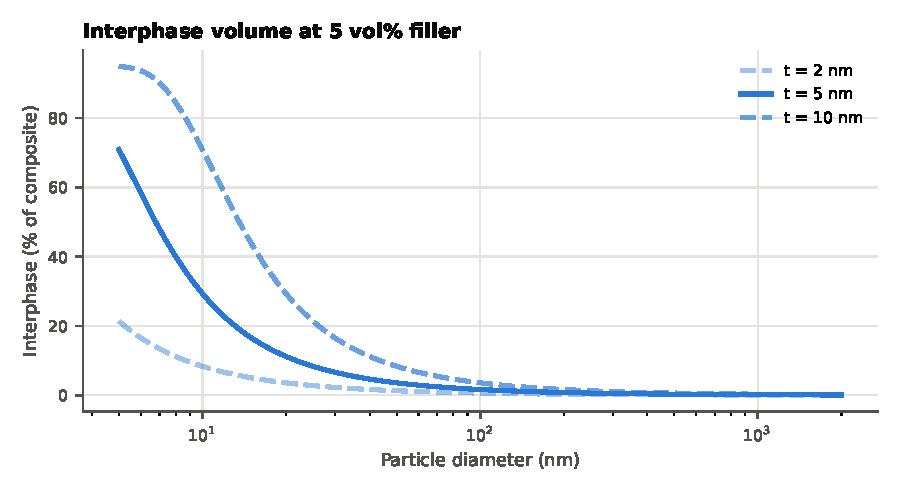
\includegraphics[width=0.82\textwidth]{fig1_interphase.pdf}
\caption{Model-predicted interphase volume fraction (Eq.~\ref{eq:phii}) versus particle diameter at 5~vol\% loading for assumed shell thicknesses of 2, 5 and 10~nm.}
\label{fig:interphase}
\end{figure}
For a 5~nm shell at 5~vol\%, the interphase occupies 11.2\% of the composite for 20~nm particles, 29.3\% for 10~nm particles and 0.15\% for 1~$\mu$m particles (Fig.~\ref{fig:interphase}). Particles 20~nm in diameter are then on average 24~nm apart. These are geometric consequences of the assumed shell. Whether the shell is a physically distinct region must be established experimentally.

\subsection{Permittivity and local field}
\begin{figure}[htbp]
\centering
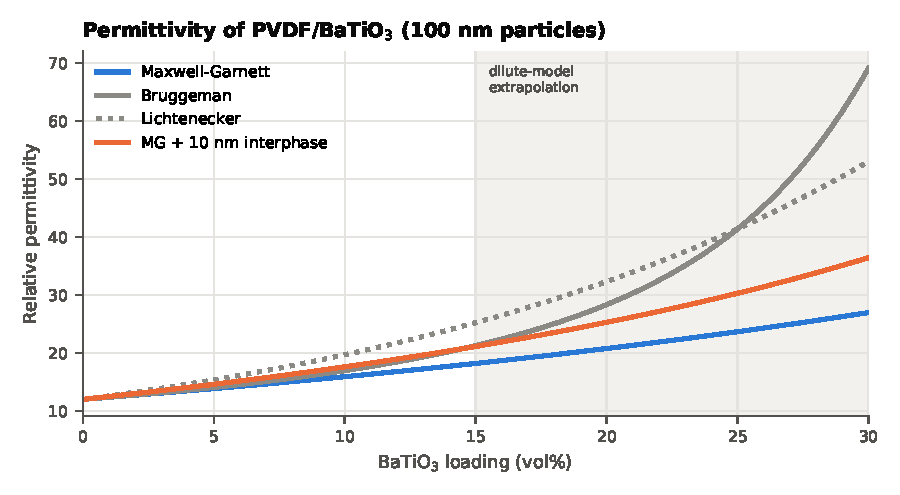
\includegraphics[width=0.82\textwidth]{fig2_permittivity.pdf}
\caption{Model-predicted relative permittivity of PVDF/\BTO{} (100~nm particles). The shaded region marks the loading range where dilute-model predictions are extrapolations.}
\label{fig:perm}
\end{figure}

\begin{table}[htbp]
\centering
\caption{Model-predicted relative permittivity of PVDF/\BTO{} (100~nm particles; interphase $t=10$~nm, $\varepsilon_i=30$).}
\label{tab:perm}
\small
\begin{tabular}{rcccc}
\toprule
\BTO{} (vol\%) & Maxwell--Garnett & Bruggeman & Lichtenecker & MG + interphase \\
\midrule
5 & 13.9 & 14.1 & 15.4 & 14.6 \\
10 & 15.9 & 17.0 & 19.7 & 17.6 \\
20$^\dagger$ & 20.8 & 28.3 & 32.3 & 25.3 \\
30$^\dagger$ & 27.0 & 69.1 & 53.0 & 36.4 \\
\bottomrule
\multicolumn{5}{l}{\footnotesize $^\dagger$Qualitative extrapolation beyond the dilute range.}
\end{tabular}
\end{table}

Up to 10~vol\%, the four models agree within about 25\%, and the predicted permittivity remains far below that of \BTO{} (Table~\ref{tab:perm}, Fig.~\ref{fig:perm}). Under the dilute-sphere model, a \BTO{} particle sees a small fraction of the average field: $L_E=0.021$ in the dilute limit and 0.028 at 10~vol\%, against 1.09 for ZnO. The stress coefficient is favourable for both ($L_T=2.42$ for \BTO{}, 2.44 for ZnO). Within this model, therefore, the direct contribution of an unpoled or weakly poled high-permittivity filler is small. Real particles with non-spherical shapes, contacts or conductive pathways can experience substantially different local fields.

\subsection{Poling direction}
\begin{figure}[htbp]
\centering
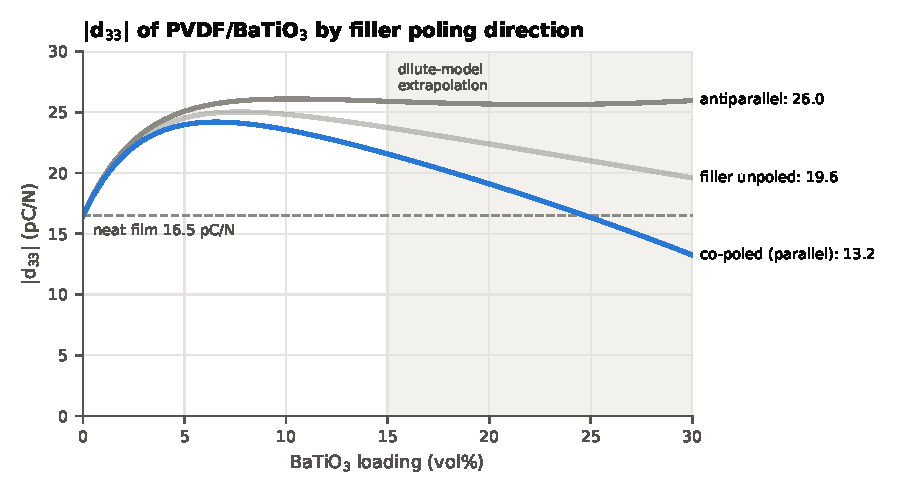
\includegraphics[width=0.82\textwidth]{fig3_poling.pdf}
\caption{Model-predicted $|\dt|$ of PVDF/\BTO{} versus loading for three filler poling configurations (nominal nucleation scenario).}
\label{fig:poling}
\end{figure}
In the nominal nucleation scenario, all three poling cases rise from 16.5 to about 24--26~pC/N by 6--8~vol\% (Fig.~\ref{fig:poling}). The rise comes from the assumed increase in $\Fp$. At 10~vol\%, the predicted $|\dt|$ is 26.1 (antiparallel), 24.8 (unpoled filler) and 23.6~pC/N (co-poled). In the extrapolated range at 30~vol\%, co-poling lowers $|\dt|$ to 13.2~pC/N, below the unfilled film.

\subsection{Sensitivity to the nucleation law}\label{sec:sens}
\begin{figure}[htbp]
\centering
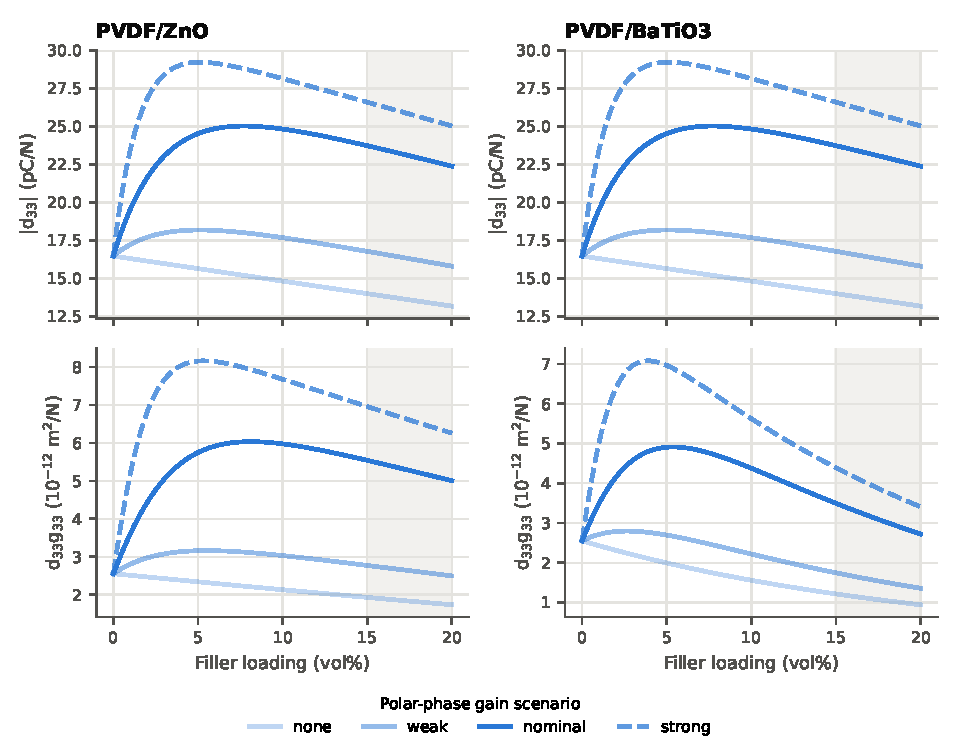
\includegraphics[width=0.9\textwidth]{fig4_nucleation_sensitivity.pdf}
\caption{Model-predicted $|\dt|$ (top) and $\dt g_{33}$ (bottom) for PVDF/ZnO and PVDF/\BTO{} (filler unpoled) under the four nucleation scenarios of Table~\ref{tab:scen}.}
\label{fig:sens}
\end{figure}
The nucleation law controls the predictions (Fig.~\ref{fig:sens}, Table~\ref{tab:senstab}). Without a polar-phase gain, adding either filler lowers $|\dt|$, because it dilutes the piezoelectric matrix. Both fillers give the same $|\dt|$ in all scenarios, because the unpoled filler term is zero and the nucleation law is the same for both. Their figures of merit differ only through permittivity. For \BTO{}, a weak polar-phase gain still gives a lower figure of merit than the unfilled film ($2.22$ vs $2.55\times10^{-12}$~m$^2$/N); for ZnO it gives a higher one ($3.03$).

\begin{table}[htbp]
\centering
\caption{Model-predicted response at 10~vol\% loading (filler unpoled) for each nucleation scenario. Unfilled film: $|\dt|=16.5$~pC/N, $\dt g_{33}=2.55\times10^{-12}$~m$^2$/N.}
\label{tab:senstab}
\small
\begin{tabular}{lccc}
\toprule
Scenario & $|\dt|$ (pC/N) & $\dt g_{33}$, ZnO ($10^{-12}$ m$^2$/N) & $\dt g_{33}$, \BTO{} ($10^{-12}$ m$^2$/N) \\
\midrule
None & 14.8 & 2.13 & 1.56 \\
Weak & 17.7 & 3.03 & 2.22 \\
Nominal & 24.8 & 5.98 & 4.38 \\
Strong & 28.1 & 7.68 & 5.63 \\
\bottomrule
\end{tabular}
\end{table}

\subsection{Particle size}
\begin{figure}[htbp]
\centering
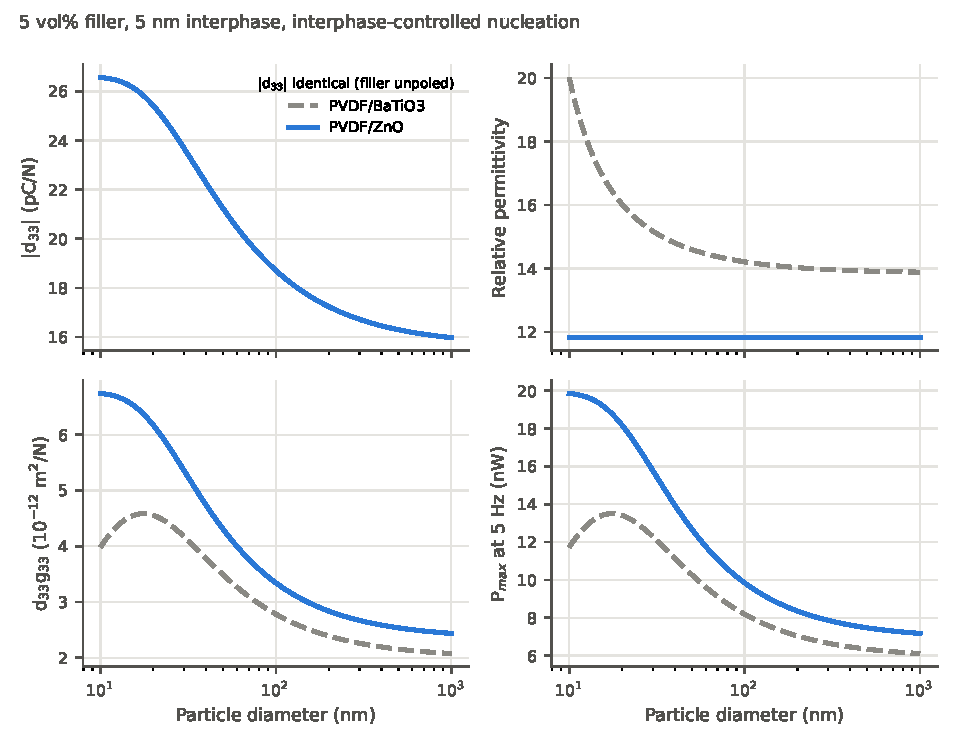
\includegraphics[width=0.9\textwidth]{fig5_particle_size.pdf}
\caption{Model-predicted $|\dt|$, permittivity, $\dt g_{33}$ and $P_{\max}$ versus particle diameter at 5~vol\%, with nucleation tied to interphase volume (Eq.~\ref{eq:lawi}; $t=5$~nm, $\Delta F=0.35$, $\phi_{i,\mathrm{sat}}=0.05$). Interphase permittivity: $\varepsilon_i=\varepsilon_m$ for ZnO, $\varepsilon_i=30$ for \BTO{}.}
\label{fig:size}
\end{figure}
When nucleation is tied to interphase volume, the predicted response depends strongly on particle size (Fig.~\ref{fig:size}). For PVDF/ZnO, the figure of merit rises from $2.44\times10^{-12}$ at 1~$\mu$m to $6.74\times10^{-12}$~m$^2$/N at 10~nm. Over the same range, $P_{\max}$ rises from 7.2 to 19.9~nW. For PVDF/\BTO{}, the figure of merit peaks at $4.59\times10^{-12}$~m$^2$/N near 17~nm and then falls. Below that size, the high-permittivity interphase raises the composite permittivity (to 20.0 at 10~nm) faster than nucleation raises $\dt$. Particles below 10~nm are not shown: there, the coated-sphere volume approaches close packing and the model no longer applies.

\subsection{Frequency and dielectric loss}\label{sec:freq}
\begin{figure}[htbp]
\centering
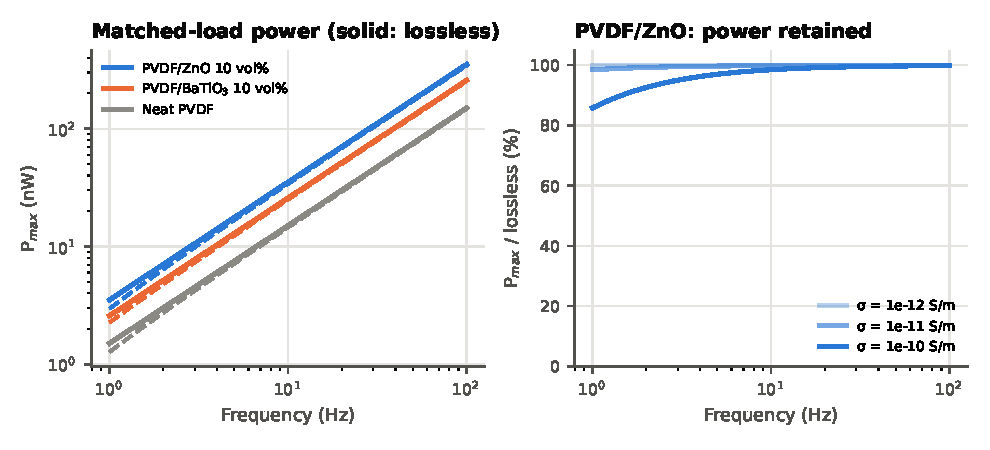
\includegraphics[width=0.95\textwidth]{fig6_frequency_loss.pdf}
\caption{Left: model-predicted matched-load power from 1 to 100~Hz without loss (solid) and with $\sigma=10^{-10}$~S/m plus $\tan\delta=0.02$ (dashed). Right: fraction of lossless power retained by PVDF/ZnO (10~vol\%) for three conductivities.}
\label{fig:freq}
\end{figure}
For a charge source under constant force amplitude, $P_{\max}\propto f$. For PVDF/ZnO, it rises from 3.5~nW at 1~Hz to 352~nW at 100~Hz (Fig.~\ref{fig:freq}). Conduction loss (Eq.~\ref{eq:tand}) acts mainly at low frequency. With $\sigma=10^{-10}$~S/m plus $\tan\delta=0.02$, the composite retains 84\% of its lossless power at 1~Hz and 98\% at 100~Hz. For $\sigma\le10^{-11}$~S/m, the loss in power is below 2\% at all frequencies. Under matched load, loss mainly lowers the optimum resistance and the stored charge. A semiconducting filler that raises composite conductivity toward $10^{-10}$~S/m or above would penalise slow, body-motion harvesting more than vibration harvesting.

\subsection{Device output}
\begin{table}[htbp]
\centering
\caption{Model-predicted device performance under assumed parameters: 2~cm $\times$ 2~cm, 60~$\mu$m film, 50~N, 5~Hz, filler unpoled, nominal nucleation scenario, 10~vol\% filler.}
\label{tab:device}
\small
\resizebox{\textwidth}{!}{\begin{tabular}{lccccccc}
\toprule
Film & $\dt$ & $\varepsilon_r$ & $\dt g_{33}$ & $V_{oc}$ & $R_{\mathrm{opt}}$ & $P_{\max}$ & $P_{\max}$, $\tan\delta=0.05$ \\
 & (pC/N) & & ($10^{-12}$ m$^2$/N) & (V) & (M$\Omega$) & (nW) & (nW) \\
\midrule
PVDF/ZnO composite & $-24.8$ & 11.7 & 5.98 & 1.81 & 46.3 & 17.6 & 16.7 \\
PVDF/\BTO{} composite & $-24.8$ & 15.9 & 4.38 & 1.32 & 33.9 & 12.9 & 12.3 \\
Unfilled PVDF ($\Fp=0.50$) & $-16.5$ & 12.0 & 2.55 & 1.16 & 44.9 & 7.5 & 7.2 \\
\bottomrule
\end{tabular}}
\end{table}
For the assumed particle properties and equal polar-phase content, the PVDF/ZnO composite has a higher predicted $\dt g_{33}$, $V_{oc}$ and $P_{\max}$ than the PVDF/\BTO{} composite (Table~\ref{tab:device}). The two composites have the same $\dt$. The difference comes entirely from permittivity. This is a controlled model comparison. Real ZnO and \BTO{} particles also differ in surface chemistry, morphology, agglomeration, conductivity, defect chemistry and nucleation efficiency, so the comparison does not establish that one filler is generally superior.

\subsection{Parameter sensitivity}
\begin{figure}[htbp]
\centering
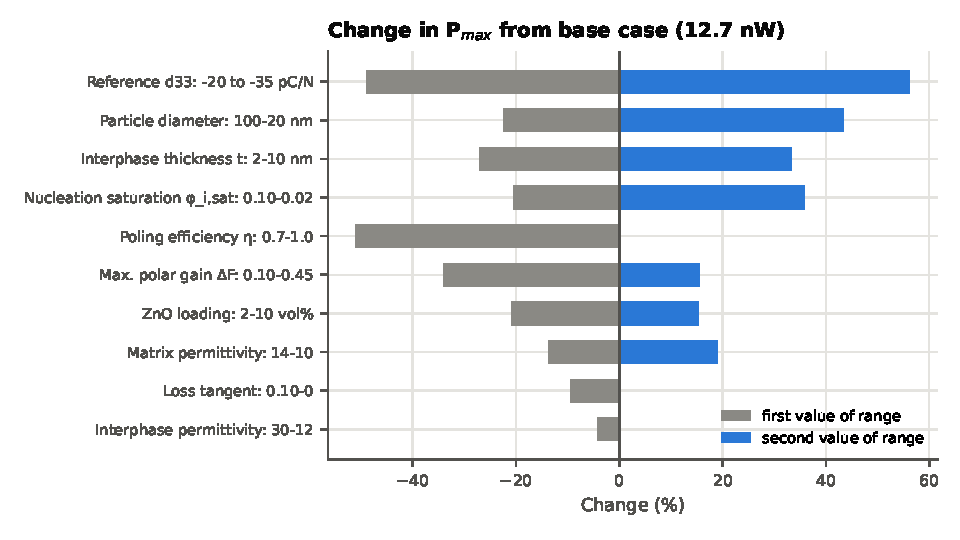
\includegraphics[width=0.85\textwidth]{fig7_tornado.pdf}
\caption{One-at-a-time sensitivity of model-predicted $P_{\max}$ for PVDF/ZnO (50~nm, 5~vol\%, interphase-controlled nucleation; base case 12.7~nW). Bars show the change when each parameter is set to the first or second value of its range.}
\label{fig:tornado}
\end{figure}
Fig.~\ref{fig:tornado} ranks the parameters by their effect on $P_{\max}$. The largest are the reference matrix coefficient ($-49$\% to $+56$\%) and poling efficiency (down to $-51$\% at $\eta=0.7$). The next group comprises the parameters that control nucleation: particle diameter ($-22$\% to $+43$\%), nucleation saturation ($-21$\% to $+36$\%), interphase thickness ($-27$\% to $+33$\%) and maximum polar gain ($-34$\% to $+16$\%). Loss tangents up to 0.1 and interphase permittivity (for ZnO) change $P_{\max}$ by 10\% or less. The parameters that most need measurement are therefore the matrix $\dt$, the poling efficiency, and the nucleation response of the specific filler.

%=====================================================================
\section{Validation protocol}\label{sec:valid}
The framework is not yet validated against experiment. The assumed inputs are designed to be replaced by measurements as follows.
\begin{enumerate}
\item Measure FTIR (763, 840, 1234, 1275~cm$^{-1}$) and DSC for at least four loadings, and compute $F(\beta)$, $F(\gamma)$ and $X_c$ with Eq.~\eqref{eq:fea} ff.
\item Fit Eq.~\eqref{eq:law} to the measured $\Fp(\phi)$ with the provided least-squares routine (\texttt{nucleation.\allowbreak fit\_\allowbreak saturating\_\allowbreak law}). Use the fitted law, not the scenarios, in Eq.~\eqref{eq:d33}.
\item Measure $\varepsilon'(\omega)$ and $\tan\delta(\omega)$ from 0.1~Hz to 1~MHz, and compare with the effective\-/medium predictions to bound $\varepsilon_i$ and $t$.
\item Measure quasi-static $\dt$ on poled samples. Compare it with Eq.~\eqref{eq:d33} using measured $X_c$ and $\Fp$, with $\eta$ as the only free parameter.
\item Measure $V_{oc}$ and $P(R)$ under controlled force, area and frequency. Include a polarity-reversal test to exclude triboelectric signals.
\end{enumerate}
Agreement in step 4 with a physically reasonable $\eta$ would support the claim that polar-phase content dominates. Systematic underprediction for piezoelectric fillers would instead point to a larger direct filler contribution or to interfacial space-charge effects.

%=====================================================================
\section{Discussion}

\paragraph{Design implications.} Within the assumptions of the framework, the following implications follow. They should be tested experimentally.
\begin{enumerate}
\item Smaller, well-dispersed particles maximise interphase volume. Agglomerates behave as large particles and introduce voids.
\item The nucleation response of the filler and the matrix poling efficiency matter more than the filler's own $\dt$. Surface chemistry, which sets surface charge, is therefore a primary variable.
\item A low permittivity mismatch favours both field coupling during poling and $g_{33}$. High-permittivity piezoceramics need antiparallel or high-field poling to contribute directly.
\item Co-poling a positive-$\dt$ filler with PVDF reduces the composite response. The poling sequence and direction should be reported.
\item Harvesters should be compared by $\dt g_{33}$ and lossy matched-load power, with force, area, frequency, thickness and load stated.
\end{enumerate}

\paragraph{Limitations.} The model is first-order. The dilute-sphere coupling coefficients ignore particle interaction, shape, percolation and imperfect bonding. The matrix term neglects crystal orientation and the amorphous contribution to the sign of $\dt$, and it weights $\beta$ and $\gamma$ equally. The nucleation laws are phenomenological and assumed. Space-charge electret effects, the size-dependent loss of tetragonality in \BTO{} nanoparticles~\cite{Hoshina2008}, mechanical resonance and nonlinear contact mechanics are not included. The material parameters are representative, not measured.

\paragraph{Open problems.} Open problems include separating nucleation, intrinsic filler response, space-charge and triboelectric contributions in measured output. Direct measurement of interphase thickness, permittivity and polarization is also needed, for example by AFM-IR, piezoresponse force microscopy or Kelvin-probe microscopy. Other open problems are the long-term stability of polarization and space charge under humidity, temperature and $10^6$--$10^8$ loading cycles, and links from atomistic simulations of surface--chain interactions to continuum electromechanics.

%=====================================================================
\section{Conclusions}
We developed a first-order modeling framework that links PVDF phase content, interphase geometry, dielectric mixing, poling configuration and lossy harvester output. Within the parameter range considered, it indicates that changes in matrix polar-phase content can outweigh the directly transmitted response of high-permittivity fillers. That conclusion depends on the nucleation law, which must be measured for each filler system. Without a polar-phase gain, the model predicts that fillers lower $\dt$.

The model also predicts several further trends. Co-poling positive-$\dt$ fillers reduces the composite response. Smaller particles help PVDF/ZnO monotonically, but PVDF/\BTO{} shows an optimum size near 17~nm. Conduction loss matters mainly at low frequency. The open implementation and validation protocol allow these predictions to be tested directly against FTIR, DSC, dielectric and device measurements.

\section*{Code and data availability}
The \texttt{pvdf\_nano} package (version 0.2.0), the unit tests, the script that reproduces every figure and table, and the generated data files are available at \url{https://github.com/subrahmanyamtanala-rgb/PVDF-Metal-Oxide-Nanocomposites-}. [Archive DOI and license to be added.]

%=====================================================================
\begin{thebibliography}{99}
\small
\bibitem{Lovinger1983} A.~J. Lovinger, Ferroelectric polymers, \emph{Science} \textbf{220} (1983) 1115--1121.
\bibitem{Gregorio1994} R.~Gregorio Jr., M.~Cestari, Effect of crystallization temperature on the crystalline phase content and morphology of poly(vinylidene fluoride), \emph{J. Polym. Sci. B: Polym. Phys.} \textbf{32} (1994) 859--870.
\bibitem{Martins2014} P.~Martins, A.~C. Lopes, S.~Lanceros-Mendez, Electroactive phases of poly(vinylidene fluoride): determination, processing and applications, \emph{Prog. Polym. Sci.} \textbf{39} (2014) 683--706.
\bibitem{Cai2017} X.~Cai, T.~Lei, D.~Sun, L.~Lin, A critical analysis of the $\alpha$, $\beta$ and $\gamma$ phases in poly(vinylidene fluoride) using FTIR, \emph{RSC Adv.} \textbf{7} (2017) 15382--15389.
\bibitem{Tanaka2005} T.~Tanaka, M.~Kozako, N.~Fuse, Y.~Ohki, Proposal of a multi-core model for polymer nanocomposite dielectrics, \emph{IEEE Trans. Dielectr. Electr. Insul.} \textbf{12} (2005) 669--681.
\bibitem{Lewis2004} T.~J. Lewis, Interfaces are the dominant feature of dielectrics at nanometric dimensions, \emph{IEEE Trans. Dielectr. Electr. Insul.} \textbf{11} (2004) 739--753.
\bibitem{Martins2012} P.~Martins, C.~M. Costa, M.~Benelmekki, G.~Botelho, S.~Lanceros-Mendez, On the origin of the electroactive poly(vinylidene fluoride) $\beta$-phase nucleation by ferrite nanoparticles via surface electrostatic interactions, \emph{CrystEngComm} \textbf{14} (2012) 2807--2811.
\bibitem{Sebastian2016} M.~S. Sebastian \emph{et al.}, Understanding nucleation of the electroactive $\beta$-phase of poly(vinylidene fluoride) by nanostructures, \emph{RSC Adv.} \textbf{6} (2016) 113007--113015.
\bibitem{Yamada1982} T.~Yamada, T.~Ueda, T.~Kitayama, Piezoelectricity of a high-content lead zirconate titanate/polymer composite, \emph{J. Appl. Phys.} \textbf{53} (1982) 4328--4332.
\bibitem{Katsouras2016} I.~Katsouras \emph{et al.}, The negative piezoelectric effect of the ferroelectric polymer poly(vinylidene fluoride), \emph{Nat. Mater.} \textbf{15} (2016) 78--84.
\bibitem{Furukawa1989} T.~Furukawa, Piezoelectricity and pyroelectricity in polymers, \emph{IEEE Trans. Electr. Insul.} \textbf{24} (1989) 375.
\bibitem{Ploss2000} B.~Ploss, B.~Ploss, F.~G. Shin, H.~L.~W. Chan, C.~L. Choy, Pyroelectric or piezoelectric compensated ferroelectric composites, \emph{Appl. Phys. Lett.} \textbf{76} (2000) 2776--2778.
\bibitem{Hoshina2008} T.~Hoshina, S.~Wada, Y.~Kuroiwa, T.~Tsurumi, Composite structure and size effect of barium titanate nanoparticles, \emph{Appl. Phys. Lett.} \textbf{93} (2008) 192914.
\bibitem{Wang2006} Z.~L. Wang, J.~Song, Piezoelectric nanogenerators based on zinc oxide nanowire arrays, \emph{Science} \textbf{312} (2006) 242--246.
\end{thebibliography}

\end{document}
